\documentclass[tikz,border=10pt]{standalone}
\usetikzlibrary{calc}
\begin{document}
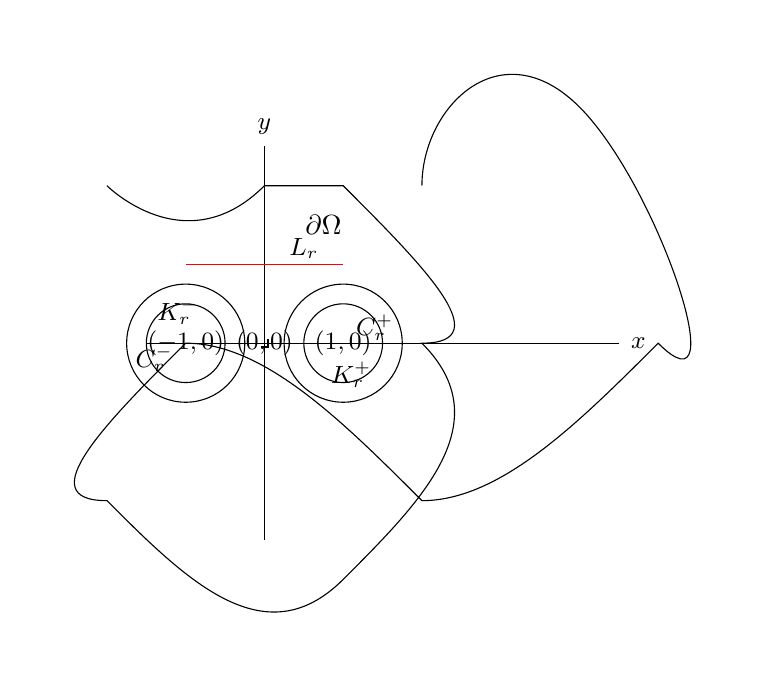
\begin{tikzpicture}[>=latex]

% The outer boundary
\draw (2,2) .. controls (2,3) and (3,4) .. (4,3) .. controls (5,2) and (6,-1) .. (5,0) .. controls (4,-1) and (3,-2) .. (2,-2) .. controls (1,-1) and (0,0) .. (-1,0) .. controls (-2,-1) and (-3,-2) .. (-2,-2) .. controls (-1,-3) and (0,-4) .. (1,-3) .. controls (2,-2) and (3,-1) .. (2,0) .. controls (3,0) and (2,1) .. (1,2) -- (0,2) .. controls (-1,1) and (-2,2) .. (-2,2);

% Axes
\draw[-] (-1.5,0) -- (4.5,0);
\draw[-] (0,-2.5) -- (0,2.5);

% Label for the x-axis
\node at (4.75,0) {\small $x$};
% Label for the y-axis
\node at (0,2.75) {\small $y$};

% The boundary of the domain
\node at (0.75,1.5) {$\partial\Omega$};
\draw[thick] (0.05,0.05) -- (0.05,-0.05) -- (-0.05,-0.05) ; % tiny dot at origin

% The circles
\draw (1,0) circle (0.75cm);
\node at (1.4,0.2) {\small $C_{r}^{+}$};
\draw (1,0) circle (0.5cm);
\node at (1.1,-0.4) {\small $K_{r}^{+}$};
\draw (-1,0) circle (0.5cm);
\node at (-1.1,0.4) {\small $K_{r}^{-}$};
\draw (-1,0) circle (0.75cm);
\node at (-1.4,-0.2) {\small $C_{r}^{-}$};

% The line L_r
\draw[red] (-1,1) -- (1,1);
\node at (0.5,1.2) {\small $L_{r}$};

% The points
\node at (-1,0) {\small $(-1,0)$};
\node at (1,0) {\small $(1,0)$};
\node at (0,0) {\small $(0,0)$};

\end{tikzpicture}
\end{document}